% Bab III  Metode Penelitian
\chapter{METODE PENELITIAN}

\section{Lokasi dan Waktu Penelitian}
Penelitian dilaksanakan di Laboratorium Jaringan Komputer, Program Studi Rekayasa Sistem Komputer, Fakultas Teknik, Universitas Muhammadiyah Buton, Baubau. Waktu pelaksanaan penelitian adalah November 2026 sampai Maret 2027.

\section{Alat dan Bahan}
Peralatan yang digunakan adalah sebuah komputer dengan prosesor 8 inti, memori 16 GB, dan sistem operasi Ubuntu 22.04 LTS. Perangkat lunak yang digunakan adalah simulator ns-3 (ns-3 Consortium, t.t.) versi 3.40 untuk simulasi, serta Python 3 untuk pengolahan data dan penyusunan grafik. Penelitian ini tidak memerlukan bahan habis pakai.

\section{Tahapan Penelitian}
Tahapan penelitian dilakukan secara berurutan seperti pada Gambar 3.1, yaitu studi literatur, perancangan skenario, implementasi pada ns-3, simulasi, pengumpulan data, dan analisis.

\begin{figure}[H]
\centering
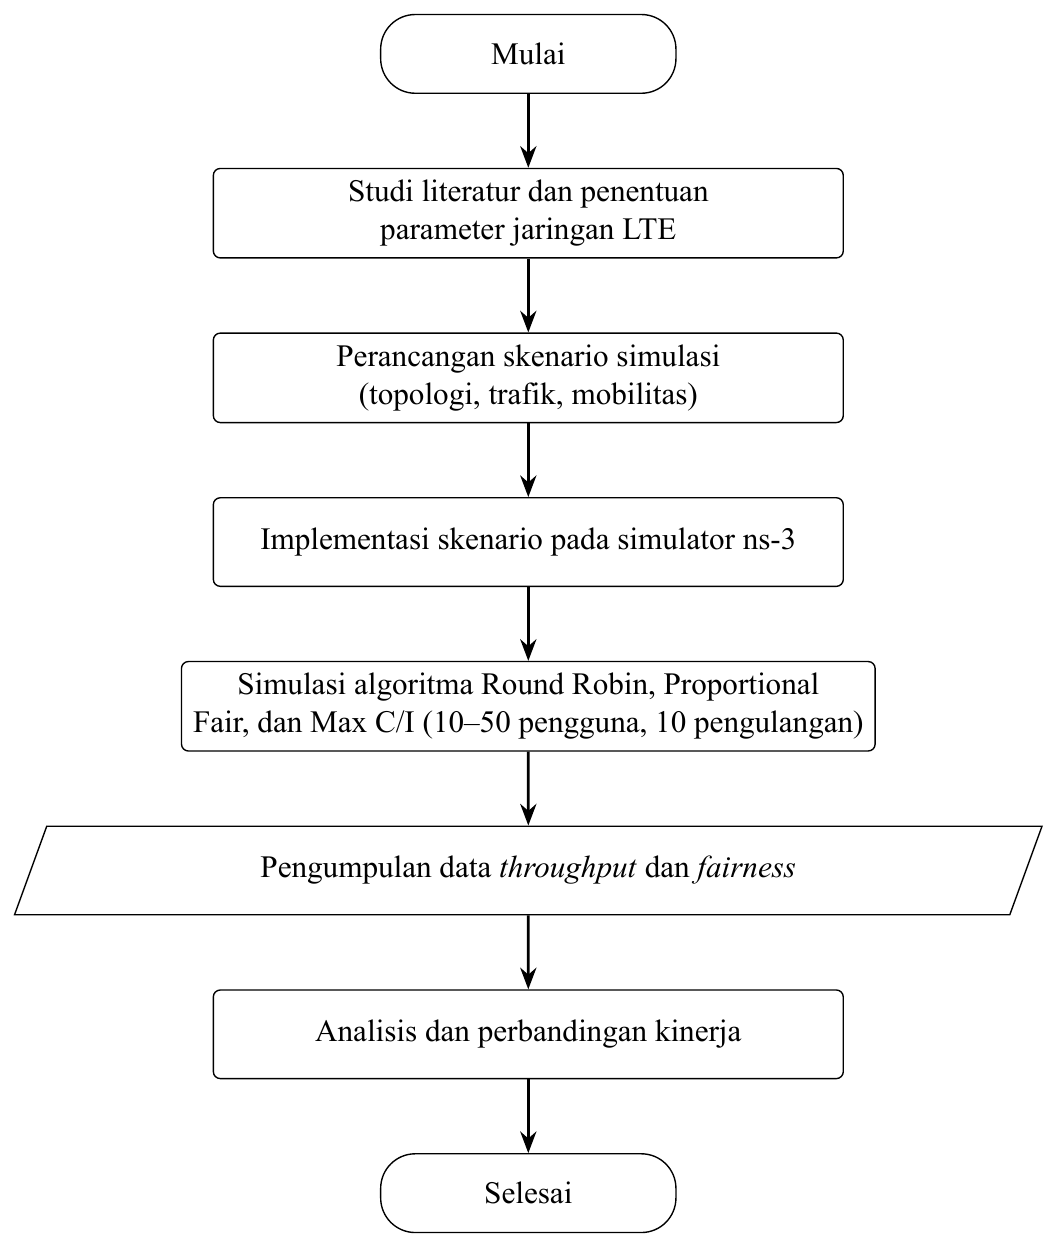
\includegraphics[width=0.52\textwidth]{../gambar/alur-penelitian.png}
\caption{Diagram alir tahapan penelitian}
\end{figure}

\section{Perancangan Skenario Simulasi}
Skenario simulasi terdiri atas satu eNodeB di pusat sel dengan radius 500 m dan sejumlah pengguna (UE) yang tersebar acak dan bergerak seperti pada Gambar 3.2. Parameter simulasi digunakan sesuai Tabel 3.1.

\begin{figure}[H]
\centering
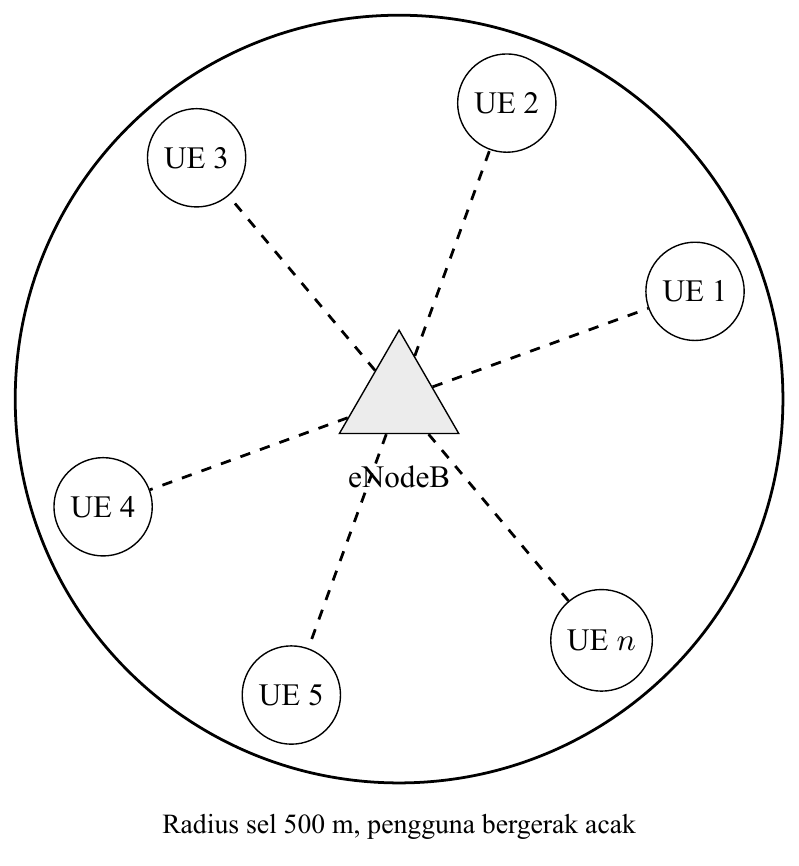
\includegraphics[width=0.45\textwidth]{../gambar/topologi.png}
\caption{Topologi simulasi satu sel LTE}
\end{figure}

\begin{singlespace}
\begin{longtable}{|p{0.42\linewidth}|p{0.46\linewidth}|}
\caption{Parameter simulasi}\\
\hline
\textbf{Parameter} & \textbf{Nilai} \\
\hline
Lebar pita \textit{downlink} & 20 MHz (100 RB) \\
\hline
Jumlah eNodeB & 1 \\
\hline
Radius sel & 500 m \\
\hline
Jumlah pengguna (UE) & 10, 20, 30, 40, 50 \\
\hline
Model mobilitas & \textit{Random walk}, kecepatan 3 km/jam \\
\hline
Model propagasi & Friis \\
\hline
Trafik & UDP \textit{downlink}, paket 1.024 byte, 1 Mbps per UE \\
\hline
Algoritma penjadwalan & RR, PF, Max C/I \\
\hline
Durasi simulasi & 60 detik \\
\hline
Pengulangan & 10 kali dengan \textit{seed} berbeda \\
\hline
\end{longtable}
\end{singlespace}

\section{Variabel dan Analisis Data}
Variabel bebas penelitian adalah algoritma penjadwalan (RR, PF, Max C/I) dan jumlah pengguna (10--50). Variabel terikatnya adalah \textit{throughput} total (Mbps) dan indeks \textit{fairness} Jain. Setiap kombinasi algoritma dan jumlah pengguna disimulasikan 10 kali dengan \textit{seed} acak berbeda, kemudian dihitung nilai rata-ratanya. Perbandingan antaralgoritma dinyatakan dalam persentase selisih terhadap algoritma RR sebagai acuan, dan disajikan dalam tabel dan grafik.
